\documentclass[9pt,a4paper,twocolumn,notitlepage]{article}
\usepackage[margin=0.9in]{geometry}
\usepackage{hyperref}
\usepackage[final]{pdfpages}
\usepackage{subcaption}
\usepackage{cite}
\usepackage[acronym]{glossaries}
\usepackage{titling}

\setlength{\columnsep}{0.275in}

\makeglossaries

\newacronym{scc}{SCC}{Strongly Connected Components}
\newacronym{anf}{ANF}{Approximate Neighbourhood Function}
\newacronym{spid}{SPID}{Shortest Paths Index of Dispersion}

\title{An Analysis of the Portuguese Section of Wikipedia}

\author{Daniel Ramos \\ 81620 \and Miguel Tavares \\ 83528 \and Ricardo Brancas \\ 83557}

\begin{document}
\twocolumn[
\begin{@twocolumnfalse}
\maketitle
\begin{abstract}
In this report, we analyse and characterise a directed real-world network, a snapshot of the Portuguese section of Wikipedia \cite{dataset}. We explore the nature of this network and examine its behaviour with WebGraph \cite{webgraph}, a tool used to study large networks. Finally, we conclude it displays common characteristics of a scale-free network, governed by power law distributions.
\end{abstract}
\vspace{2\baselineskip}
\end{@twocolumnfalse}
]

\section{Introduction}
The goal of this project is to analyse and characterise a real world network, and to  get acquainted with tools and methods which will be useful in following endeavours.
As such, we have chosen to analyse a snapshot of the Portuguese section of Wikipedia \cite{dataset}.
We have chosen such a large network in order to get familiarised with WebGraph \cite{webgraph}.

The representation of this network consists of a node for each page, and an edge from node $x$ to node $y$ whenever page $x$ has a link to page $y$.

\section{Methods}
The tools used to make this report were WebGraph\cite{webgraph}, NumPy, Matplotlib, the \texttt{powerlaw} package\cite{alstott_bullmore_plenz_2014} and snippets of code made available
by Prof. Alexandre Francisco \cite{aplf}.

The network was originally represented as an edge list which was subsequently converted in an adjacency list (\texttt{ASCIIGraph} format), by use of a simple \texttt{C++} program, since this is the input
format for WebGraph's compression algorithms.

After running WebGraph, we used a Python script to parse the output and generate the figures present in this document.

\section{Results and Discussion}

The network we have chosen contains $1\,603\,222$ vertices (pages) and $49\,021\,409$ edges (links). Both the minimum in and out-degrees are $0$ (meaning there are pages that are not connected); the maximum in-degree is $207\,254$ while the maximum out-degree is $12\,237$. Finally the combined average degree is approximately $61.15$. Furthermore, there are 121 \acrfull{scc}, the largest being comprised of $1\,602\,960$ nodes.
\vspace{1\baselineskip}

\begin{figure}[h]
	\centering
	\begin{subfigure}{.475\textwidth}
		\centering
		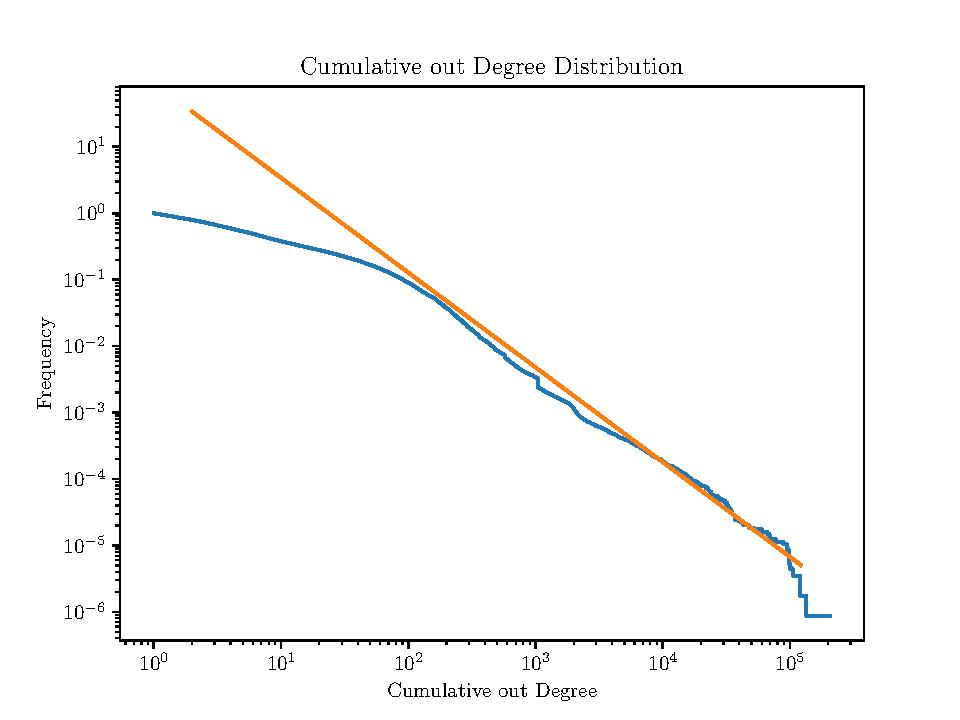
\includegraphics[width=\linewidth]{wikipedia_pt_in.pdf}
		\caption{Cumulative in-degree distribution.}
		\label{fig:inddist}
	\end{subfigure}
	\begin{subfigure}{.475\textwidth}
		\centering
		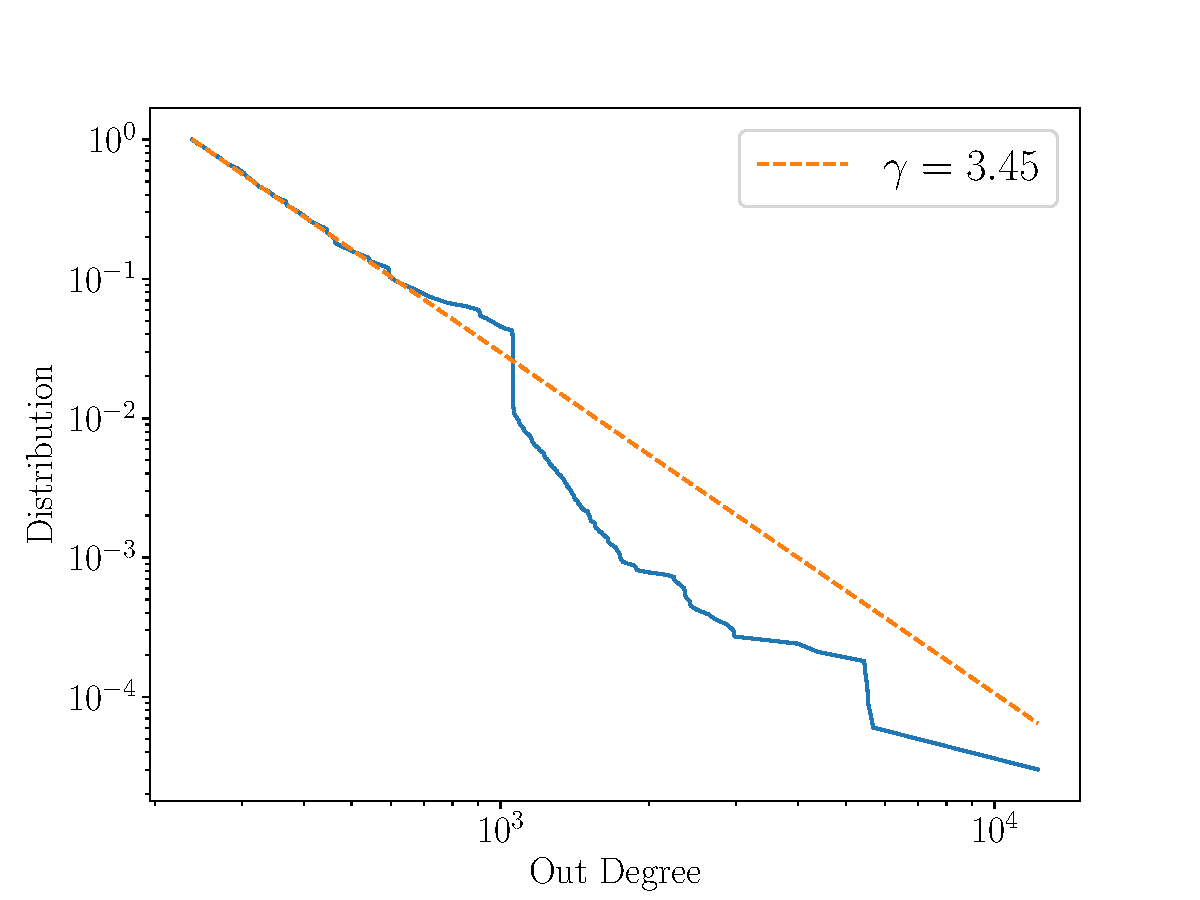
\includegraphics[width=\linewidth]{wikipedia_pt_out.pdf}
		\caption{Cumulative out-degree distribution.}
		\label{fig:outddist}
	\end{subfigure}
	\caption{Degree distributions.}
\end{figure}

In figures ~\ref{fig:inddist} and~\ref{fig:outddist} we present the in-degree distribution and out-degree distribution, respectively, and their power-law regressions. The regressions were obtained using the \texttt{powerlaw} package \cite{alstott_bullmore_plenz_2014} through a method described by Clauset et al. \cite{Clauset2009}.

We have found that our degree distributions correlate highly with a power-law distribution, excluding the effects of low degree saturation and high degree cutoff; expected results of the finite nature of real networks.

Based on the regressions computed, we found an in-degree parameter $\gamma = 2.59$ that is lower than its out-degree counterpart $\gamma = 3.45$. This difference in parameters helps explain the disparity between the maximum out-degree and the maximum in-degree. Although our data is unlabelled, we believe this phenomenon occurs because there are few Wikipedia pages which are referenced by most of the others, leading to a higher maximum degree on the in-degree distribution. Conversely, the out-degree distribution has a lower maximum degree, because it is uncommon for a single page to reference a lot of other pages (the number of references per page is within a shorter interval). This can be explained through the idea of popularity: when someone writes a new page, the references they will create are not entirely random, instead they are biased towards the most popular pages, that they already know.
The out-degree distribution has a lower $\gamma$ because it is more dispersed than the in-degree distribution, meaning that the difference in frequency between high-degree and low-degree nodes is less accentuated in the in-degree distribution.

The variance for the in-degree distribution is $206\,082.30$. This result is also expected, since the power-law distribution has a $\gamma = 2.59$ implying a divergent variance for an infinite set. The variance of the out-degree distribution is significantly lower at $6\,296.66$, which is also expected, since a $\gamma = 3.45$ implies a finite variance, hence the lower value.

\begin{figure}[h]
	\centering
	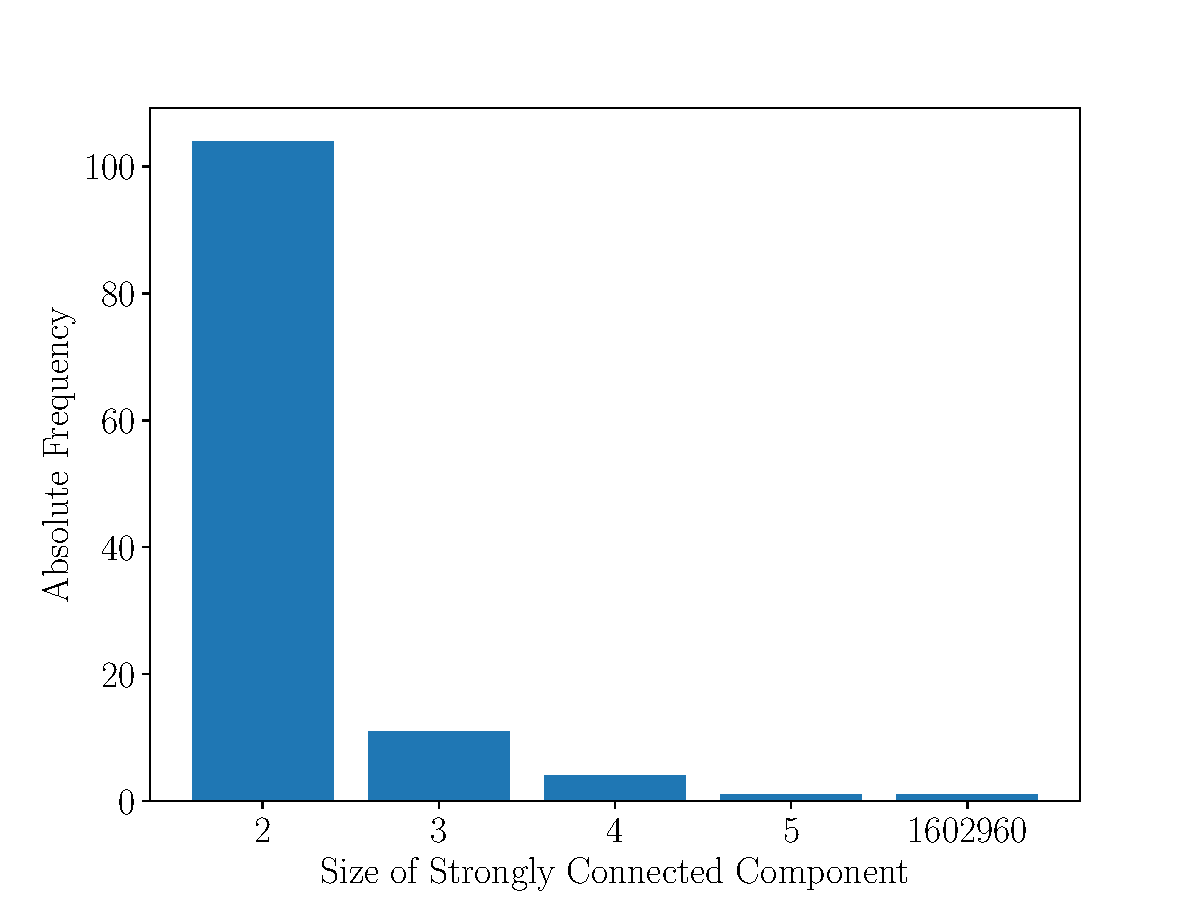
\includegraphics[width=\linewidth]{wikipedia_pt_sccdistr.pdf}
	\caption{Strongly Connected Component distribution.}
	\label{fig:sccdist}
\end{figure}

Figure \ref{fig:sccdist} shows the number of \acrshort{scc}s in respect to their cardinality. We notice a giant strongly connected component, as expected, containing almost all the nodes ($1\,602\,960$) in the graph, and also a very few small ones. These results are in accordance with the expected results if the network were a random graph, as the average degrees obtained ($> ln(N)$) imply a connected regime. However our graph is not connected, and as such it is impossible to compute the diameter through the usual method. Thus we used the effective diameter, a more robust measure that calculates the diameter using $90\%$ as a cut-off of the cumulative probability function. We obtained an effective diameter of $5.8361 \pm 0.0022$. An alternative and even more significant measure is the Harmonic Diameter \cite{fogaras}, which we learned to be $6.8982 \pm 0.0403$. This indicator uses the harmonic sum in order to account for the possibility of non connected pages.

\begin{figure}[h]
	\centering
	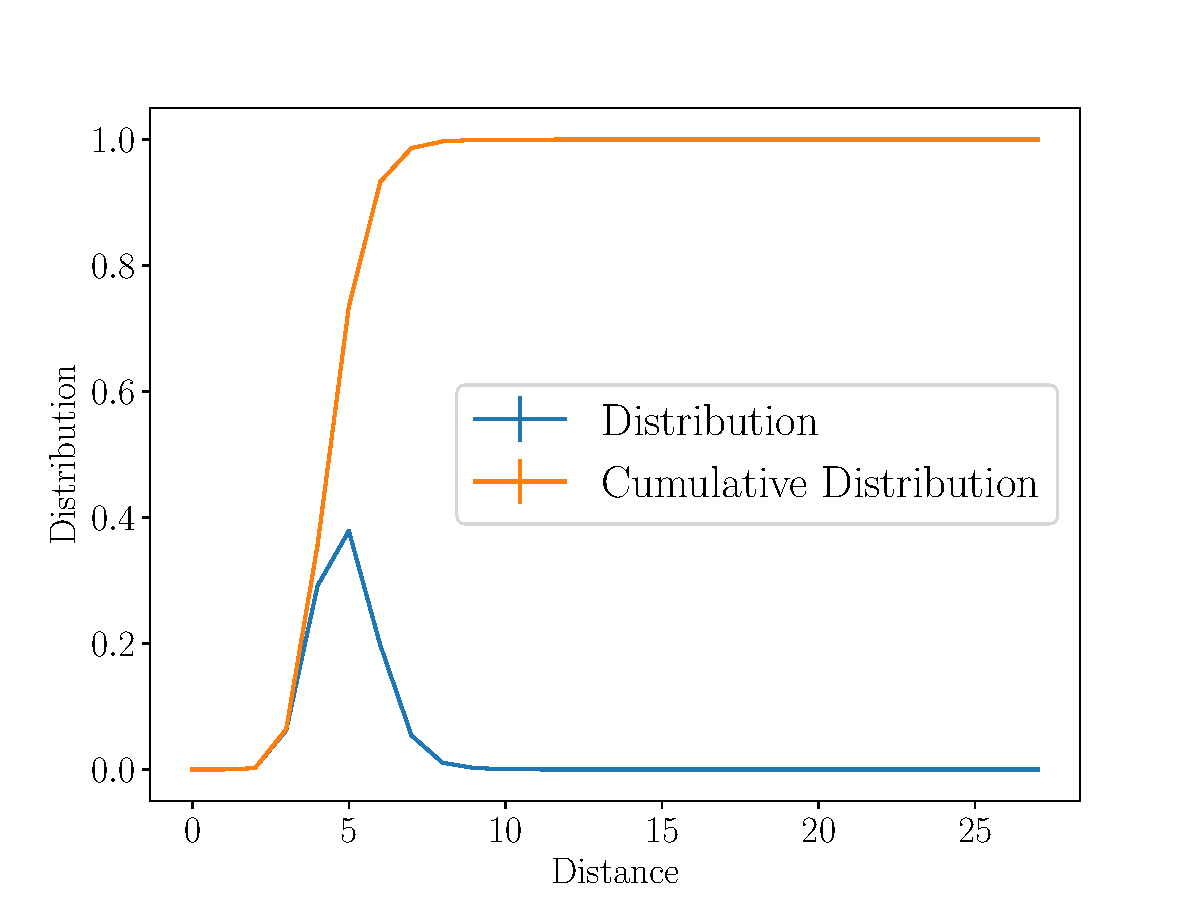
\includegraphics[width=\linewidth]{wikipedia_pt_neighbourhood_function.pdf}
	\caption{Approximate neighbourhood function.}
	\label{fig:neighfun}
\end{figure}

We also computed the \acrfull{anf} through WebGraph. This measure represents for each $t \in N$, the number of pairs of nodes $ \langle x, y \rangle $ such that $y$ is reachable from $x$ in less than $t$ hops \cite{Boldi2011HyperANFAT}. Since the algorithm computes an approximation, we decided to average 7 independent executions using JackKnife.
In figure \ref{fig:neighfun} we present the results; the errors for each data point are also plotted although they are too small to be seen.

We have also obtained an estimation of the Average Path Length through HyperBall\cite{DBLP:conf/icdm/BoldiV13} and JackKnife. The estimated value is $ 4.9290 \pm 0.0026 $. This result is in accordance with the values observed in Figure~\ref{fig:neighfun}: roughly a half of the nodes can be reached from each other in just 5 hops. As such, we conclude the Portuguese Wikipedia page's to have approximately 5 degrees of separation, on average. Considering, again, that the network were a random network, the expected Average Path Length would be $\frac{ln(n)}{ln(k)} = 4.2$, which is not too far from the obtained value.


\begin{figure}[h]
	\centering
	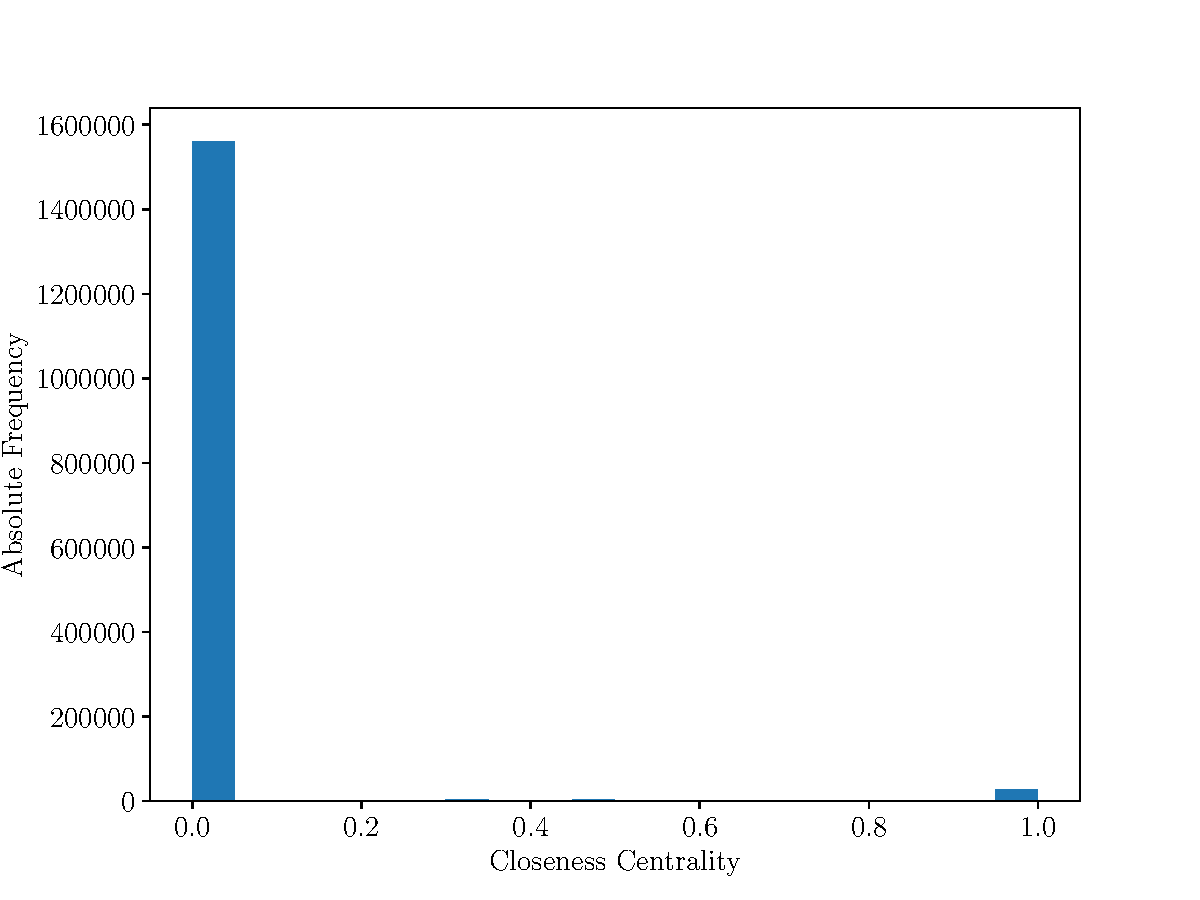
\includegraphics[width=\linewidth]{wikipedia_pt_closeness_centrality.pdf}
	\caption{Closeness centrality.}
	\label{fig:closeness}
\end{figure}

\begin{figure}[h]
	\centering
	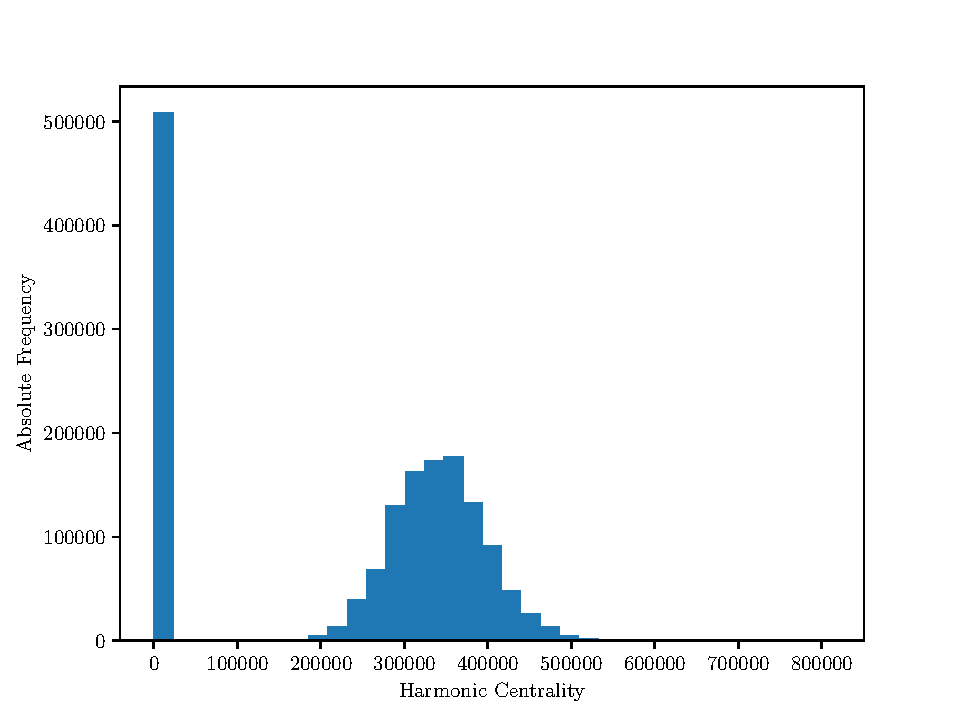
\includegraphics[width=\linewidth]{wikipedia_pt_harmonic_centrality.pdf}
	\caption{Harmonic centrality.}
	\label{fig:harmonic}
\end{figure}

Out of curiosity we decided to estimate the closeness centrality, and the results are just as expected. As it can be seen in Figure~\ref{fig:closeness} almost all nodes have a closeness centrality of 0, this is due to our graph not being connected. Since this measure does not give us any further information on the graph, we also decided to calculate the harmonic centrality, which nicely allows the existence of disconnected nodes by giving them less weight than to the closer vertices, which means their contribution is close to 0. Figure~\ref{fig:harmonic} exhibits the obtained results. If a node had an harmonic centrality of $1$, it would mean it was just at 1 hop of any other node. In Figure~\ref{fig:harmonic} we can observe there are $465\,301$ nodes isolated from the rest of the network, the remaining nodes have an average harmonic centrality of $0.22$. We also note that there are $465\,279$ unreachable nodes the maximum harmonic centrality for any node would be $$1-\frac{465\,279}{1\,603\,222}=0.7098$$
a value two times higher than that of the maximum obtained.

We have also verified a \acrfull{spid} of $0.2287 \pm 1.9232 \times 10^{-4}$, which according to Boldi et al. \cite{Boldi2011HyperANFAT} correlates to a ``properly social" network.

\section{Conclusion}

In short we conclude that the Portuguese section of Wikipedia displays the common characteristcs of a scale free network, governed by a power law with $\gamma = 2.59$ for the in-degree distribution and $\gamma = 3.45$ for the out-degree distribution, the difference between these values being typical of Internet samples.

We have also verified that Wikipedia's pages are usually strongly connected witch a very small distance between each other, excluding a few outliers that are generally not connected at all.

\printglossary[type=\acronymtype]

\bibliographystyle{plain}
\bibliography{references}

\end{document}
